\documentclass[aspectratio=149]{beamer}

\usepackage[utf8]{inputenc}
\usepackage[T1]{fontenc}

\usepackage[english]{babel}
\usepackage{amsmath}
\usepackage{cleveref}
\usepackage{amssymb}
\usepackage{mathtools}

%%Numbers, expectation
\newcommand{\N}{\mathbb{N}}
\newcommand{\E}{\mathbb{E}}
\renewcommand{\P}{\mathbb{P}}
\newcommand{\Var}{\mathbb{V}}
\newcommand{\R}{\mathbb{R}}
\newcommand{\D}{\mathcal{D}}
\newcommand{\B}{\mathcal{B}}
\newcommand{\Dh}{\D_h}
\renewcommand{\phi}{\varphi}
\newcommand*\diff{\mathop{}\!\mathrm{d}} % integral

%% mathoperator
\DeclareMathOperator*{\argmax}{arg\,max}
\DeclareMathOperator*{\argmin}{arg\,min}
\DeclareMathOperator*{\dom}{dom}
\DeclareMathOperator*{\sign}{sign}
\DeclareMathOperator*{\diag}{diag}

\DeclareMathOperator*{\Cov}{Cov}
\DeclareMathOperator*{\Cor}{Corr}
\DeclareMathOperator*{\Id}{Id}

%proximal operator
\newcommand{\prox}[3][]{\operatorname{prox}^{#1}_{#2}\left(#3 \right)}

\usepackage{xcolor}

%% sort citations by increasing number
\usepackage[sort,nocompress]{cite}

\usepackage{graphicx}% http://ctan.org/pkg/graphicx
\graphicspath{{../figures/}{../../figures}{../../memes}} %Setting the graphicspath
\usepackage{caption,subcaption}

\usepackage{tikz}
\usepackage{pgfplots}
\usetikzlibrary{backgrounds}
\usetikzlibrary{intersections}
\usepgfplotslibrary{fillbetween}

% \usepackage[right]{showlabels}


%%
\theoremstyle{plain}
\newtheorem{prop}{Proposition}[section]
\newtheorem{algo}{Algorithm}[section]
\newtheorem{assumption}{Assumption}
\theoremstyle{remark}
\newtheorem{remark}{Remark}[section]

% cref
\crefname{assumption}{Assumption}{Assumptions}
\crefname{equation}{}{}

\usepackage{autonum}

\usepackage{bm} %% bold math symbols

\usepackage{bbm} %% for \mathbbm{1}


% algorithmic environment
\usepackage{algorithm}
\usepackage[noend]{algpseudocode}

% for some reason this was required on one void linux installation (but not the other)
\usepackage{sansmathaccent}
\pdfmapfile{+sansmathaccent.map}

\author{Axel Böhm}

% shows which section we're in
\usetheme{Darmstadt}

% page number
\setbeamertemplate{footline}[frame number]
\setbeamercolor{page number in head/foot}{fg=gray}


% display things like onslide or visible already before but grayed out
\setbeamercovered{transparent}

% set the itemize item symbol as a diamond
\setbeamertemplate{itemize item}{$\diamond$}
% set the itemize subitem symbol as a triangle
\setbeamertemplate{itemize subitem}{$\blacktriangleright$}

% set the enumerate item symbol as a roman numbers
\setbeamertemplate{enumerate item}{(\roman{enumi})}


\author{Axel Böhm}

% shows which section we're in
\usetheme{Darmstadt}

% page number
\setbeamertemplate{footline}[frame number]
\setbeamercolor{page number in head/foot}{fg=gray}


% display things like onslide or visible already before but grayed out
\setbeamercovered{transparent}

% set the itemize item symbol as a diamond
\setbeamertemplate{itemize item}{$\diamond$}
% set the itemize subitem symbol as a triangle
\setbeamertemplate{itemize subitem}{$\blacktriangleright$}

% set the enumerate item symbol as a roman numbers
\setbeamertemplate{enumerate item}{(\roman{enumi})}


% reference: https://yuxinchen2020.github.io/ele522_optimization/lectures/variance_reduction.pdf
% or
% https://ieeexplore-ieee-org.uaccess.univie.ac.at/stamp/stamp.jsp?tp=&arnumber=9226504

\usepackage{booktabs}

\title{Duality, Gradient-free, in Application}
\date{\today}

\begin{document}
\maketitle
\frame{\tableofcontents}


\section{Duality}%

\begin{frame}
  \frametitle{Duality}
  \begin{center}
    Establishes some relation between two classes of objects.
  \end{center}
  \begin{definition}[``Legendre transform'' or ``Fenchel conjugate'']
    Given a function $f: \R^d \to \R \cup \{+\infty\}$, we define its \textcolor{blue}{\textbf{conjugate}} $f^*:\R^d \to \R \cup\{+\infty\}$ by
    \begin{equation}
      f^*(y) = \sup_x \{\langle y,x \rangle - f(x)\}
    \end{equation}
  \end{definition}
\end{frame}

\begin{frame}
  \frametitle{Convex conjugate}

  \begin{block}{}
    \begin{equation}
      f^*(y) = \sup_x \{\langle y,x \rangle - f(x)\}
    \end{equation}
  \end{block}
  \begin{minipage}{0.48\textwidth}
  \begin{figure}[ht]
    \centering
    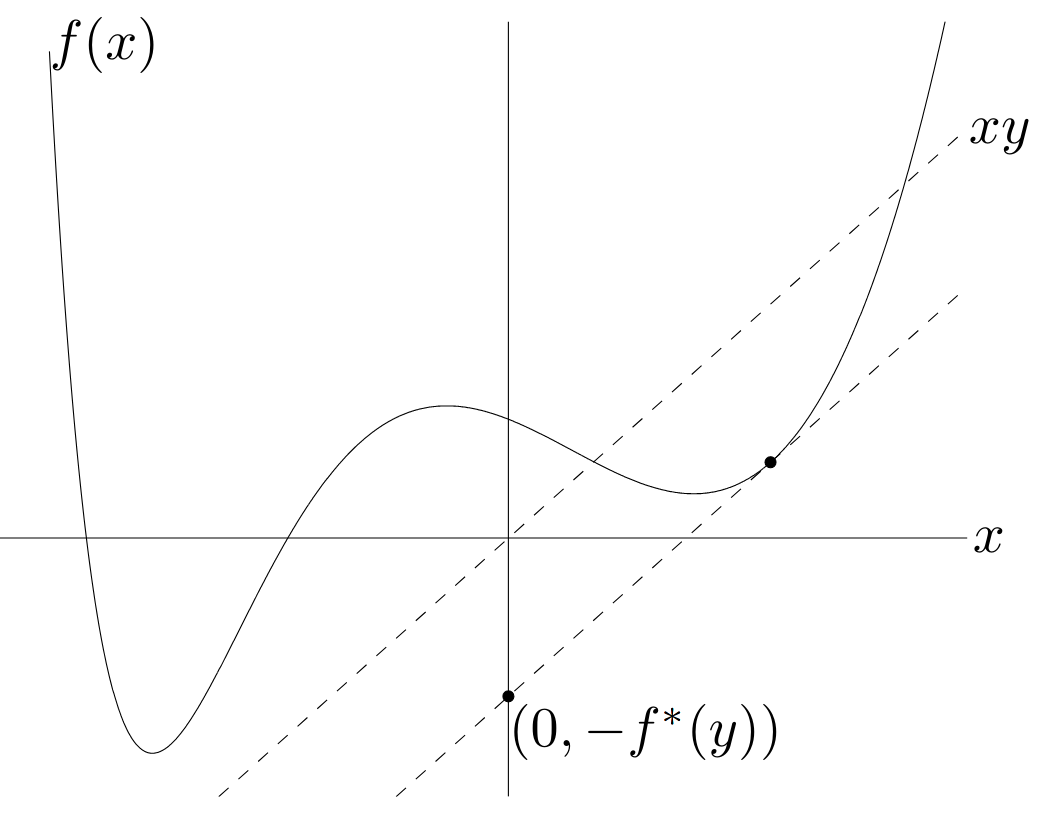
\includegraphics[width=\textwidth,keepaspectratio]{conjugate}
  \end{figure}
  \end{minipage}
  \begin{minipage}{0.48\textwidth}
    \vspace{2cm}
    \textcolor{blue}{Figure:} maximum gap between linear function $x \mapsto \langle y, x \rangle$ and $f$
  \end{minipage}
\end{frame}

\begin{frame}
  \frametitle{Properties}

  \begin{itemize}
    \item $f^*$ is always convex. \hfill{\textcolor{gray}{point-wise max of affine function}}
    \item \textcolor{blue}{Fenchel's inequality:}
          \begin{equation}
            f(x) + f^*(y) \ge \langle x, y \rangle.
          \end{equation}
    \item Hence the biconjugate $f^{**}:={(f^*)}^*$ satisfies $f^{**}\le f$.
    \item If f is convex an lsc. then $f^{**}=f$.
    \item etc.
  \end{itemize}
\end{frame}

\begin{frame}
  \frametitle{Examples}
  \begin{itemize}
    \item \textcolor{blue}{Norm:} If $f(x) = \Vert x \Vert$, then
          \begin{equation}
            f^*(y) = \mathbbm{1}(\Vert y \Vert_* \le 1),
          \end{equation}
          i.e.\ the indicator of the dual norm ball.
          Recall the definition of the dual norm:
          \begin{equation}
            \Vert y \Vert_* :=  \max_{\Vert x \Vert \le 1} \{\langle y, x \rangle\}.
          \end{equation}
          In particular: $\Vert \cdot \Vert_1 \leftrightarrow \Vert \cdot \Vert_\infty$
  \end{itemize}
\end{frame}

\begin{frame}
  \frametitle{More examples}
    \begin{equation}
      \hspace{-4cm}\text{\textcolor{blue}{Generalized linear models:}}  \qquad \min_{x\in \R^d} \, f(Ax) + g(x).
    \end{equation}
    Two approaches to reformulate:
    \begin{equation}
      \min_x \underbrace{\max_y \, \langle y, Ax \rangle - f^*(y)}_{= f(Ax)} + g(x).
    \end{equation}
    Switch min and max
    \begin{equation}
      \min_x \max_y \, - f^*(y) + \langle y, Ax \rangle + g(x).
    \end{equation}
    Change sign to go from max to min
    \begin{equation}
      \min_x \, - f^*(y) - \min_y \underbrace{-\langle y, Ax \rangle - g(x)}_{= g^*(-A^T y)}.
    \end{equation}
\end{frame}

\begin{frame}
  \frametitle{Generalized linear models continued}
  Or reformulate
  \begin{equation}
    \min_{x\in \R^d} \, f(Ax) + g(x)
  \end{equation}
  as
  \begin{equation}
    \min_{x\in\R^d, w\in \R^m} \, f(w)+ g(x) \quad \text{s.t.} w = Ax
  \end{equation}
  Use Lagrange function
  \begin{equation}
    \mathcal{L}(x,w, u) :=  \, f(w)+ g(x) \langle u, w - Ax \rangle,
  \end{equation}
  then the dual function is given by
  \begin{equation}
    \varphi(u) = \min_{x\in\R^d, w\in \R^m} \mathcal{L}(x,w,u).
  \end{equation}
  Dual problem
  \begin{equation}
    \max_{u \in \R^m} [\varphi(u) = - f^*(-u) - g^*(A^T u)].
  \end{equation}
\end{frame}


\begin{frame}
  \frametitle{Example: Lasso}
  $\ell_1$ regularized regression
  \begin{equation}
    \min_{x\in \R^d}\, \frac12 \Vert Ax-b \Vert^2 + \lambda \Vert x \Vert_1
  \end{equation}
  fits this template with
  \begin{equation}
    f(w) = \frac12 \Vert w-b \Vert^2 \quad \text{and} \quad g(x) = \lambda \Vert x \Vert_1
  \end{equation}
  Computation gives
  \begin{equation}
    f^*(u) = \frac12 \Vert b \Vert^2 - \frac12 \Vert b-u \Vert^2 \quad \text{and} \quad g^*(v)= \mathbbm{1}(\Vert v/\lambda \Vert_\infty \le 1).
  \end{equation}
\end{frame}

\begin{frame}
  \frametitle{Dual of Lasso}
  We had
  \begin{equation}
    f^*(u) = \frac12 \Vert b \Vert^2 - \frac12 \Vert b-u \Vert^2 \quad \text{and} \quad g^*(v)= \mathbbm{1}(\Vert v/\lambda \Vert_\infty \le 1).
  \end{equation}
  So the dual is
  \begin{equation}
    \begin{aligned}
      &\max_{u\in \R^m} - f^*(-u) - g^*(A^T u) \\
      \Leftrightarrow& \min_{u\in\R^m} \Vert b+u \Vert^2 \quad \text{s.t.} \quad \Vert A^T u \Vert_{\infty} \le \lambda
    \end{aligned}
  \end{equation}

  Similarly, for least squares, ridge/logistic regression, SVM, etc.
\end{frame}

\begin{frame}
  \frametitle{But why?}
  \begin{itemize}
    \item Duality gap gives a \textcolor{blue}{certificate} of current optimization quality
          \begin{equation}
            \begin{aligned}
              f(A \bar{x}) + g(\bar{x}) &\ge \min_{x\in\R^d} \, f(Ax) + g(x) \\
              & \ge \max_{u\in\R^m} - f^*(-u) - g^*(A^T u) \\
              &\ge -f^*(-\bar{u}) - g^*(A^T \bar{u})
            \end{aligned}
          \end{equation}
    \item Stopping criterion
    \item Dual problem is sometimes easier to solve
  \end{itemize}
\end{frame}


\section{Derivative free}%
\label{sec:}


\begin{frame}
  \frametitle{}

  \begin{center}
    \Huge\textcolor{blue}{Zero-order Optimization}\\
    $\Leftrightarrow$ \textcolor{blue}{Derivative-Free}\\
    $\Leftrightarrow$ \textcolor{blue}{Blackbox}
  \end{center}


\end{frame}

\begin{frame}
  \frametitle{Look, no gradients!}
  Can we solve $\min_{x\in \R^d}\, f(x)$ without access to gradients?

  \begin{algorithm}[H]
    \caption{Random search}
    \begin{algorithmic}[1]
      \For{$k = 1,2, \dots$}
      \For{pick a random direction $d_k \in \R^d$}
      \State{$\gamma_k:= \argmin_{\gamma\in \R} f(x_k+ \gamma d_k)$}
      \State{$x_{k+1} := x_k+ \gamma_k d_k$}
      \EndFor{}
    \end{algorithmic}
  \end{algorithm}

\end{frame}

\begin{frame}
  \frametitle{Convergence rate for derivative-free random search}
  Converges same as gradient descent - up to a slow-down factor $d$.

  \textcolor{blue}{Proof.}
  \begin{equation}
    f(x_k+ \gamma d_k ) \le f(x_k) + \gamma \langle d_k, \nabla f(x_k) \rangle + \frac{\gamma^2L}{2} \Vert d_k \Vert^2
  \end{equation}
  Minimizing the upper bound (RHS), there exists a step $\bar{\gamma}$ for which
  \begin{equation}
    f(x_k + \bar{\gamma}d_k) \le f(x_k) - \frac{1}{L} \left\langle \frac{d_k}{\Vert d_k \Vert^2}, \nabla f(x_k)\right\rangle.
  \end{equation}
  So our (exact line-search) step can only be better
  \begin{equation}
    f(x_k + \gamma_k d_k) \le f(x_k + \bar{\gamma}d_k)
  \end{equation}
  Taking expectation and using $\E_r \langle r, g \rangle^2 = 1/d \Vert g \Vert^2$ for $r \sim$ sphere, gives
  \begin{equation}
    \E [f(x_k+ \gamma_k d_k)] \le E[f(x_k)] - \frac{1}{L d} \E\left[ \Vert \nabla f(x_k) \Vert^2\right].
  \end{equation}

\end{frame}

\begin{frame}
  \frametitle{Convergence rate for derivative-free random search}
  Same as what we obtained for \textcolor{blue}{gradient descent},\\
  now with an \textcolor{blue}{extra factor of $d$}. $d$ can be huge!!!\\
  \bigskip
  Similarly for other function classes
  \begin{itemize}
    \item For convex functions, we get a rate of $\mathcal{O}(\frac{d L}{\epsilon})$.
    \item For $\mu$-strongly convex functions, we get a rate of $\mathcal{O}(d \kappa \log(1/\epsilon))$.
  \end{itemize}
  Always $d$ times the complexity of gradient descent on the function class.\\
  \bigskip
  But assumed differentiability. Can also approximate the gradient.

\end{frame}

\begin{frame}
  \frametitle{Applications for derivative-free random search}

  \textcolor{blue}{Applications}
  \begin{itemize}
    \item competitive method for \textcolor{blue}{reinforcement learning}
    \item No need to store a gradient
    \item hyperparameter optimization, and other difficult e.g. discrete optimization
problems, black-box, noisy
  \end{itemize}
\end{frame}


\begin{frame}
  \frametitle{Reinforcement learning}
  \begin{equation}
    s_{k+1} = f(s_k, a_k, e_k),
  \end{equation}
  where $s_k$ is the \textcolor{blue}{state} of the system, $a_k$ is the control \textcolor{blue}{action}, and $e_t$ is some random \textcolor{blue}{noise}. We assume existence of $f$, but it is unknown.\\
  \medskip
  We search for a ``policy''
  \begin{equation}
    a_k := \pi(a_1, \dots, a_{k-1}, s_0, \dots, s_k)
  \end{equation}

  \medskip
  \textcolor{blue}{Goal:} Maximize reward
  \begin{equation}
    \begin{aligned}
       \max_{a_k}\, &\E_{e_k} \left[ \sum_{k=1}^N R_k(s_k, a_k)\right]\\
       \text{s.t.} & s_{k+1}=f(s_k, a_k, e_k)
    \end{aligned}
  \end{equation}
\end{frame}

\section{Methods in practice}%
\label{sec:}

\begin{frame}
  \frametitle{}
  \begin{center}
    \Huge\textcolor{blue}{Adaptive \& other SGD methods}\\
  \end{center}
\end{frame}

\begin{frame}
  \frametitle{Adagrad}
  An adaptive variant of SGD
  \begin{algorithm}[H]
    \caption{Adagrad}\label{label:}
    \begin{algorithmic}[1]
      \For{$k = 1, \dots$}
      \State{pick stochastic gradient $g_k$}
      \State{$[G_k]_i = \sum_{l=}^{k}([g_k]_i)^2, \quad \forall i$}
      \State{$[x_{k+1}]_i =[x_{k}]_i - \frac{\gamma}{\sqrt{[G_k]_i}}[g_k]_i,  \quad \forall i$}
      \Endfor
    \end{algorithmic}
  \end{algorithm}
  \begin{itemize}
    \item chooses an \textcolor{blue}{adaptive, coordinate-wise} learning rate
    \item strong performance in practice
    \item many variants: Adadelta, Adam, RMSprop
  \end{itemize}
\end{frame}

\begin{frame}
  \frametitle{Adam}
  A \textcolor{blue}{momentum} variant of \textcolor{blue}{Adagrad}
  \begin{algorithm}[H]
    \caption{Adam}\label{label:}
    \begin{algorithmic}[1]
      \For{$k = 1, \dots$}
      \State{pick stochastic gradient $g_k$}
      \State{$m_k = \beta_1 m_{k-1} + (1-\beta_1)g_k$ \hfill \texttt{momentum}}
      \State{$[v_k]_i = \beta_2 [v_{k-1}]_i + (1-\beta_2){([g_k]_i)}^2$ \hfill \texttt{2nd-order statistics}}
      \State{$[x_{k+1}]_i =[x_{k}]_i - \frac{\gamma}{\sqrt{[v_k]_i}}[m_k]_i,  \quad \forall i$}
      \Endfor
    \end{algorithmic}
  \end{algorithm}
  \begin{itemize}
    \item forgetting of old weights
    \item momentum (see lecture on acceleration)
    \item strong performance for certain DL problems
  \end{itemize}
\end{frame}

\begin{frame}
  \frametitle{SignSGD}
  Only use the sign (one bit) of each gradient entry: \\
  Yields a \textcolor{blue}{communication efficient} variant of SGD.
  \begin{algorithm}[H]
    \caption{SignSGD}\label{label:}
    \begin{algorithmic}[1]
      \For{$k = 1, \dots$}
      \State{pick stochastic gradient $g_k$}
      \State{$[x_{k+1}]_i =[x_{k}]_i - \gamma_k \sign([m_k]_i),  \quad \forall i$}
      \Endfor
    \end{algorithmic}
  \end{algorithm}
  \textcolor{gray}{(possible rescaling of $\gamma_k$ by $\Vert g_k \Vert_1$)}

  \begin{itemize}
    \item combats communication bottleneck for distributed training
    \item convergence issues
  \end{itemize}


\end{frame}


\end{document}
